Android Studio ist eine für das Andoid Open Source Project (kurz: AOSP) von Google entwickelte Entwicklungsumgebung auf der Basis von IntelliJ, dabei sollte beachtet werden, dass Android Studio im gegensatz zu Android OS
proprietären Code beinhaltet und somit weder Open Source ist, noch ohne Erlaubnis durch Dritte weiterverbreitet werden darf.
IntelliJ ist eine bereits bestehende propietäre Entwicklungsumgebung für Java (bzw. JVM) und Android, des weiteren kann eine Lizenz für Firmen und Webentwickler erworben werden.
Im grunde wurde Android Studio mit der hinsicht auf Applikationsentwicklung auf dem Android OS erstellt. Es beinhaltet von Haus aus notwendige, aber auch arbeitserleichternde Komponenten, wie
einen Gradle-Compiler (Notwendig) oder einen Android-Empulator (Erleichtert das testen der App auf einem Computer).\\

%FIXME rechtschreibung
Gradle ist ein Open Source Build-Tool, was im Grunde über den eigentlichen Compiler-Prgogrammen eine oberste Schicht in der Compiler-Toolchain bildet. Daher verkörpert Gradle mehrere separate aufgaben in sich und vereinfacht das kompillieren von Android Apps enorm.
Die Kernkompnenten von Gradle sind
\begin{itemize}
\item \textbf{Linker, bzw. Zusammentragen von zusätzlichen Paketen und androidspezifischen Dateien, die für das Kompillieren erforderlich sind.} Dabei werden Pakete resp. Bibliotheken von den Quellen runtergeladen, 
die man zu der Quellenliste hinzugefügt hat. Dies erleichtert das Hinzufügen von Bibliotheken wie z.B. einer Bibliothek zum herunterladen und anzeigen von Bildern, da man nur die Downloadadresse angeben muss
und sich nicht mehr um das Einbinden der Bibliothek in sein Applikationsprojekt kümmern muss.

\item \textbf{Debugger} Wie bereits beschrieben liest sich der Debugger noch vor dem Precompiler den Code durch und macht den Programmierer auf allfällige Fehler oder verbesserungen aufmerksam.

\item \textbf{Precompiler} Der Precompiler ist ein Kernbestandteil der Compiler-Toolchain. Eine Toolchain ist eine Ansammlung von Programmen, die einem helfen aus geschriebenen Code und Assets ein lauffähiges
Programm zu erstellen. Er liest jede Datei durch und bereitet sie auf die nachfolgenden Verarbeitungsprozesse vor, indem er unter anderem Kommentare entfernt, nichtgenutzte Funktionen und Variabeln entfernt, Makros ersetzt und durch die \verb include -Kontrollzequenz eingebundene Dateien einfügt. Die heutigen Precompiler bleiben aber meist nicht nur bei ihren Kernaufgaben, sondern versuchen auch den Code so weit zu verbessern,
dass er nach dem Kompilliervorgang eine geringere Laufzeit und Speicheraulastung aufweist. Dabei ist aber zu beachten dass Compiler und Precompiler sehr eng miteinander zusammenarbeiten.

\item \textbf{Compiler} Der Compiler ist wohl das bekannteste Programm aus einer klassischen Toolchain. Er sogt dafür, dass die von dem Precompiler aufbereiteten Dateien in Maschinensprache übersetzt werden.
Wie bereits in der Einleitung erwähnt rechnet der Computer Binär. Daher ist eine Datei nichts anderes als eine lange Zahl. Je nach Prozessortyp wird auch eine Zahl anders verarbeitet. Dieser unterschied liegt in der verarbeitung von Kontrollsequenzen. In diesem trivialen Beispiel soll verdeutlicht werden, wie zwei verschiedene Prozessoren ein und die selbe Zahl anders interpretieren: Der Befehl für eine additionsoperation wird hier durch 11100010 repräsentiert. Im Prozessortyp A löst dies wie gewollt eine Addition aus, hingegen im Prozessortyp B werden die nachfolgenden Bits in den Zwischenspeicher kopiert und das Programm stürtzt ab. Prozessoren haben also auch ihre eigene Sprache, die sich durch ihre Herstellung ergibt. Diese Sprache wird \textit{Befehlssatz} genannt, wohingegen der Prozessortyp \textit{Architektur} genannt wird. Jede Prozessorarchitektur hat ihren eigenen Compiler.
Im Fall von Android haben sich drei Architekturen etabiliert: armeabi-v7, Intel x86 und AMD64. Die App wird also in mehrere Sprachen übersetzt bevor sie ausgeleifert wird.
\end{itemize}

\newpage

\begin{figure}[htbp] 
  \centering
     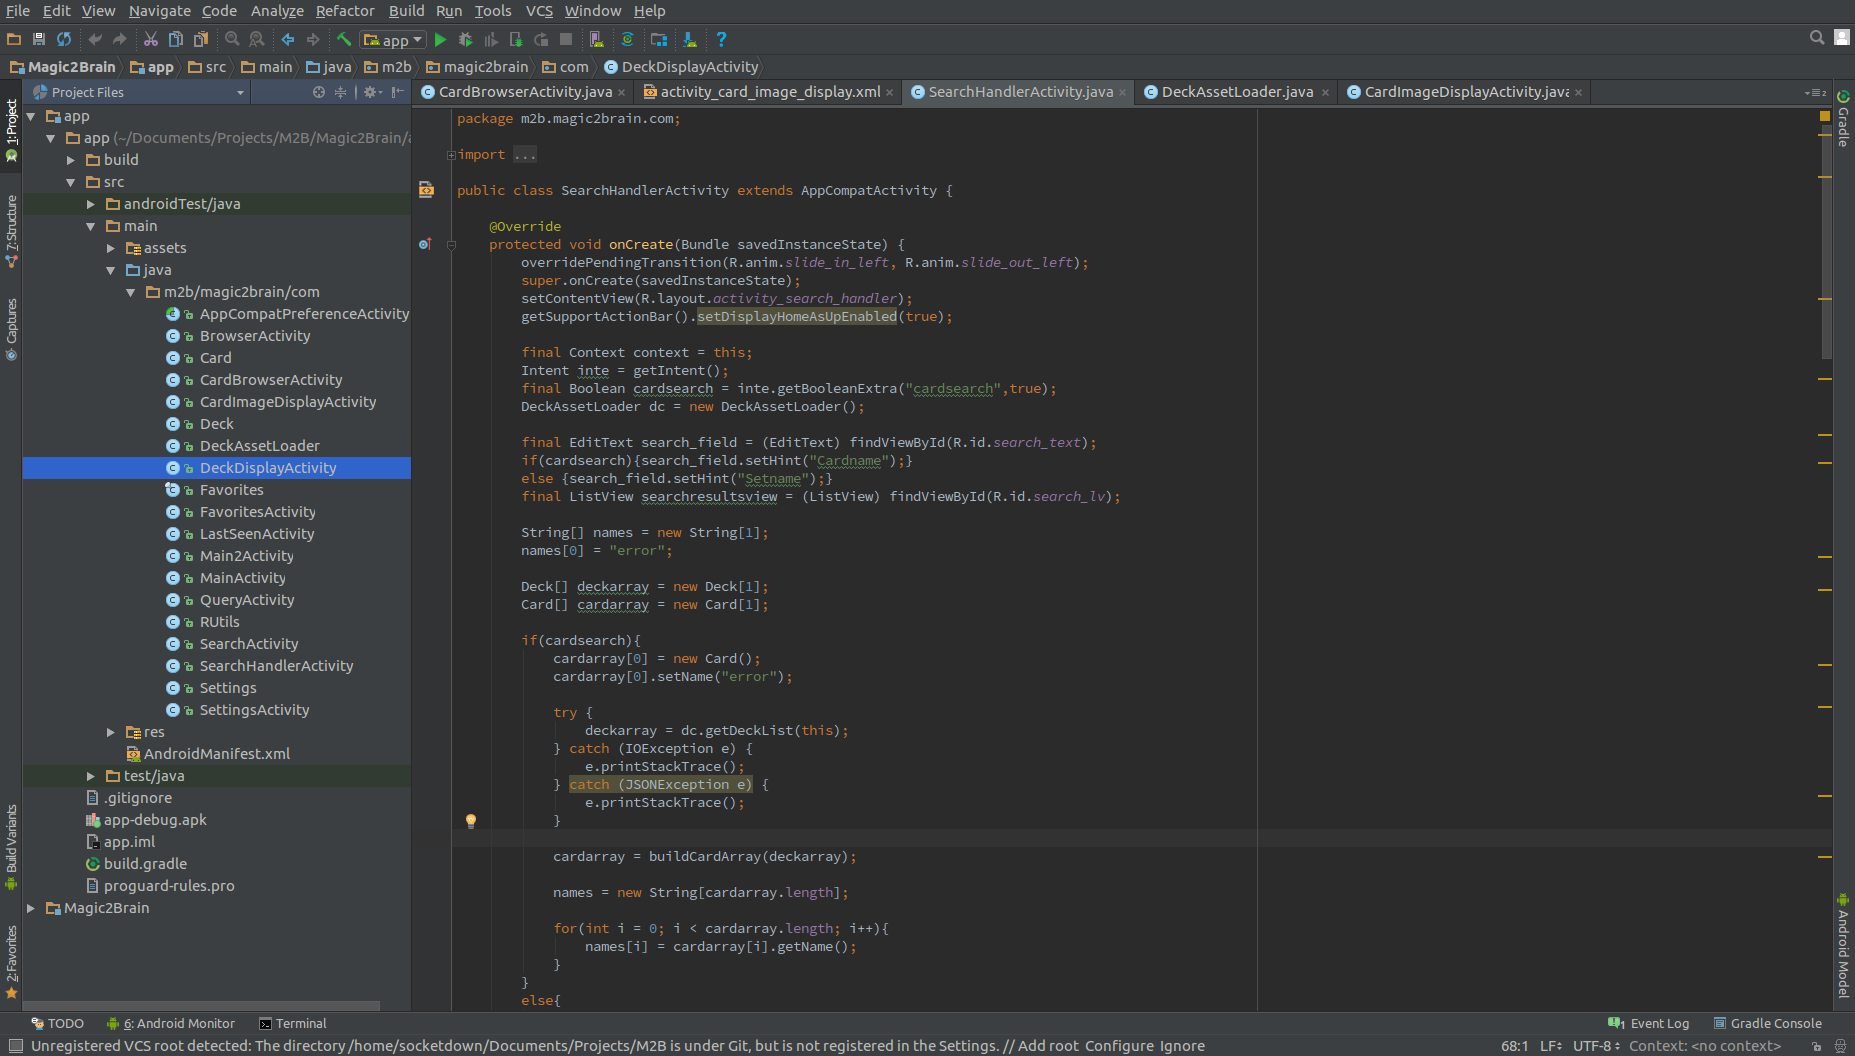
\includegraphics[width=1\textwidth]{AndroidStudio_GUI.png}
  \caption{Android Studio Benutzeroberfläche \cite{ASGUI}}
  \label{fig:Android Studio GUI}
\end{figure}
Die Grafische Benutzeroberfläche ist das Wichtigste an einer IDE. Sie erleichtert dem Entwickler die Navigation durch seinen Code in Form von Farbmarkierungen (Rechts) und Dateibrowser (Links).
Die Toolbar von Android Studio (Oben) ist mit wichtigen Shortcuts, wie z.B. Kompillierung starten, Emulator starten und Android SDK aktualisieren, gefüllt.
Der Editor von Android Studio erlaubt eine automatische Vervollständigung mit Alt+Enter. Mitunter sind auch schon fertige Vorlagen für Activities in Android Studio verfügbar, die auf Knopfdruck in das Projekt kopiert werden und gleichzeitig für die Kompillierung registirert werden. Der Dateibrowser erlaubt es zwischen Quellcode-Dateien zu wechseln und diese zur Bearbeitung zu öffnen. Zusätzlich sind Funktionen zum importieren von Dateien oder Assets vorhanden. Selbstverständlich kann dies auch manuell geschehen, indem man in einem beliebigen Dateibrowser zu dem Assets resp. Res (kurz für \textit{Ressources - dt. Ressourcen} ) - Ordner navigiert, in dem man seine Dateien ablegen kann. Mit Assets sind hier nicht Immobilien oder Vermögen gemeint, sondern Dateien, die von der App benötigt werden um richtig zu funktionnieren. Dazu gehören Bilder, Musikdateien und generell alles was kein Quellcode ist. Der IDE kann man auch Plugins hinzufügen. Plugins sind kleine Programmerweiterungen, welche dynamisch dazugeladen oder wieder entfernt werden können. Bei der Entwicklung von Magic2Brain ist das Plugin "Asset Studio" besonders nützlich gewesen, da man mit ihm Icons nicht nur in den Ressourcenordner kopieren konnte, sonder diese gleich in allen auf Android gängigen Auflösungen abspeichern konnte. Normalerweise müsste das von Hand gemacht werden, was bei unseren ca. 20 Icons sehr zeitaufwändig gewesen wäre.

\paragraph{Programmieren mit dem Android SDK}\\

Das Android SDK ist eines der wichtigsten Elemente in Android Studio. Man muss zwar nicht zwingendermassen Android Studio herunterladen, um dieses SDK zu nutzen, da es als Open Source Produkt frei verfügbar ist. Das Eigentliche Entwickeln basiert auf bereits vorgegebenen Klassen, welche man über das Klassenattribut \verb extends  mit seinem eigenen Code erweitert.
Selbstverständlch gehen dabei die herkömmlichen Progrmmiermöglichkeiten von Java nicht verloren, da es einem immernoch möglich ist eigene Klassen und Bibliotheken zu erstellen.
Eine Besonderheit von Android ist die enge Verbindung zwischen den XML-Dateien, welche Layouts, Strings und Vektorgrafiken der einzelnen Viewports enthalten.
Diese Verbindung wird einzig und allein von Gradle aufrecht erhalten. Eine aus statischen Variabeln bestehende indexierte Liste wird somit bei jedem Gradle-Build resp. bei jeder Veränderung in der Ordnerstruktur von neuem erstellt.

\paragraph{Die Bedeutung von XML Dateien für Android}\\

Das Auslagern von bestimmten Informationen in XML-Dateien ist für den erfahrenen Programmierer eine sehr schnelle, platzsparende aber auch nützliche Angelegenheit.
Somit kann er sich einige Zeilen Code sparen um ein Element einer Activity hinzuzufügen. Als Beispiel dafür wird das Erstellen eines Texteingabefeldes in einer Activity benutzt.

\begin{figure}[htbp] 
  \centering
     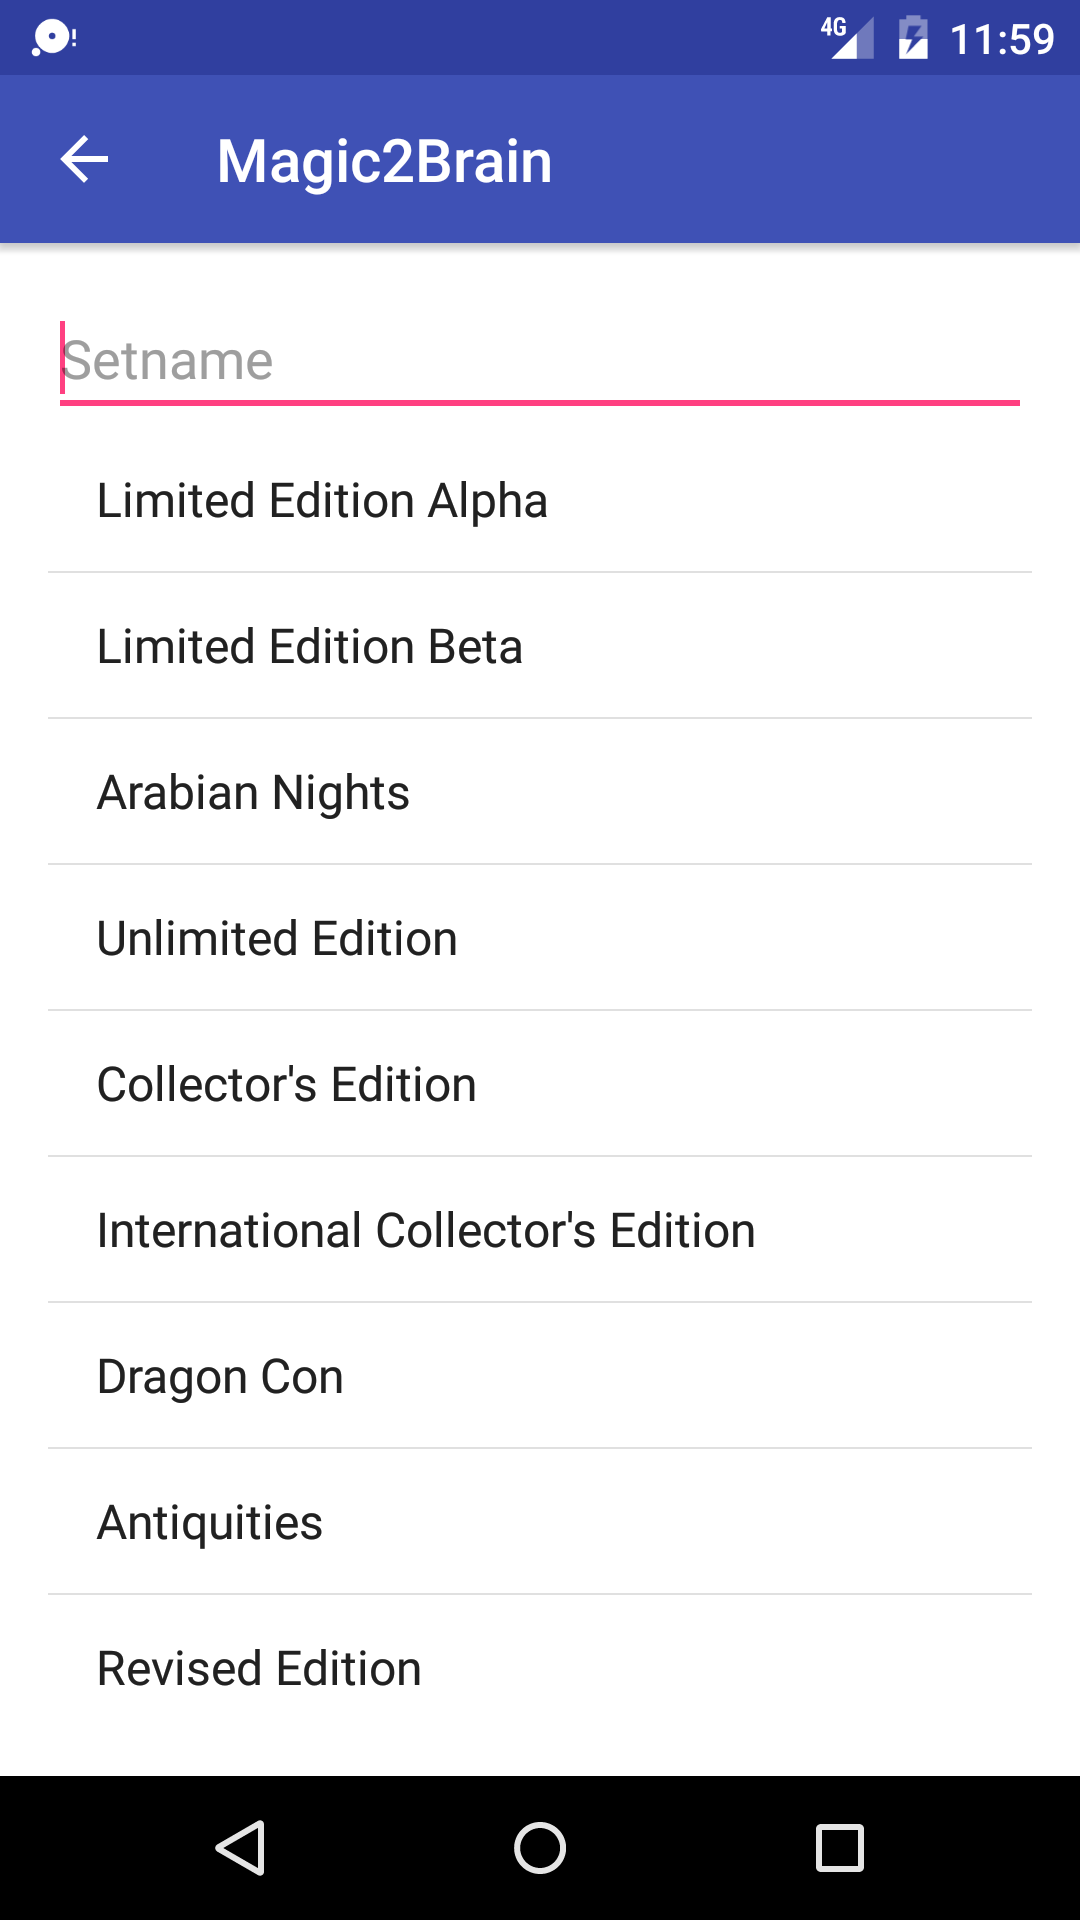
\includegraphics[width=1\textwidth]{search.png}
  \caption{Search Activity \cite{search_app}}
  \label{fig:SearchActivity}
\end{figure}

Dieses Resultat kann entweder mit XML bewerkställigt werden, aber auch mit Java selber. Im grunde ist einem diese Entscheidung selber überlassen, da das Wichtigste beim Programmieren persönliche prefärenzen sind. Dies funktionniert nach dem Schema "Solange sich der Programmierer wohl fühlt, leistet er gute Arbeit".\\

\paragraph{XML}
\begin{lstlisting}
<?xml version="1.0" encoding="utf-8"?>
<RelativeLayout xmlns:android="http://schemas.android.com/apk/res/android"
    xmlns:tools="http://schemas.android.com/tools"
    android:id="@+id/activity_search_handler"
    android:layout_width="match_parent"
    android:layout_height="match_parent"
    android:paddingBottom="@dimen/activity_vertical_margin"
    android:paddingLeft="@dimen/activity_horizontal_margin"
    android:paddingRight="@dimen/activity_horizontal_margin"
    android:paddingTop="@dimen/activity_vertical_margin"
    tools:context="m2b.magic2brain.com.SearchHandlerActivity">

    <EditText
        android:layout_width="wrap_content"
        android:layout_height="wrap_content"
        android:inputType="textPersonName"
        android:ems="10"
        android:id="@+id/search_text"
        android:layout_alignParentTop="true"
        android:layout_alignParentStart="true"
        android:layout_alignParentEnd="true"
        android:contentDescription="Name" />
</RelativeLayout>
\end{lstlisting}

Das Element "EditText" ist hier das Texteingabefeld. Im wird mit \verb android:id=  eine eindeutige ID zugewiesen, mit der später vom Code aus auf das Element zugegriffen werden kann.
In Java wird das XML folgendermassen eingebunden und auf das Element zugegriffen:
\begin{lstlisting}
//Wichtige imports werden ausgelassen
import m2b.magic2brain.com.magic2brain.R;

//Das Element wird mit der Funktion findViewByID(int ID)
//in der indexierten liste gesucht und gefunden

EditText mTextField = (EditText) findViewByID(R.id.search_text);

//nun kann mit der Variabel mTextField wie gewohnt gearbeitet werden
\end{lstlisting}

\paragraph{Java}\\
Auch bei einer puren Umsetzung in Java ist es nicht ganz möglich dem XML zu entrinnen. Um ein Objekt an einen View hinzuzufügen, muss zu allererst ein Layout verfügbar gemacht werden.
Folglich sieht das XML deutlich kürzer aus, muss aber vorhanden sein. Es muss ausserdem darauf geachtet werden, dem Layout eine ID zu geben, sonst ist es nicht möglich vom Code aus auf das Layout zuzugreifen.
\begin{lstlisting}
<?xml version="1.0" encoding="utf-8"?>
<RelativeLayout xmlns:android="http://schemas.android.com/apk/res/android"
    xmlns:tools="http://schemas.android.com/tools"
    android:id="@+id/activity_search_handler"
    android:layout_width="match_parent"
    android:layout_height="match_parent"
    android:paddingBottom="@dimen/activity_vertical_margin"
    android:paddingLeft="@dimen/activity_horizontal_margin"
    android:paddingRight="@dimen/activity_horizontal_margin"
    android:paddingTop="@dimen/activity_vertical_margin"
    tools:context="m2b.magic2brain.com.SearchHandlerActivity">
</RelativeLayout>
\end{lstlisting}

Wie bereits erwähnt besteht dieses XML nur noch aus dem rohen Layout block. \verb RelativeLayout  ist eine besondere Art von Layout, die sich hauptsächlich für Apps eignet, die später auf Endgeräten mit verschiedenen Bildschirmgössen vertrieben wird. Das einbinden in den Code geschieht wie gewohnt über \verb findViewByID(R.id.activity_search_handler);  

\begin{lstlisting}
//Imports werden hier ausgelassen

//Das Layout muss für die nachfolgenden Schritte gefunden werden
RelativeLayout lyt = (RelativeLayout) findViewById(R.id.query_absolute);

//Ein neues, unzugeordnetes Textfeld wird erstellt
EditText mTextField = new EditText(this);

//Nun wird das Textfeld zum Layout hinzugefügt
lyt.addView(mTextField);
\end{lstlisting}

Man sollte XML nur dann benutzen, wenn man wenig an seinem bisher entworfenen XML verändert. Würde man dynamisch Elemente wie z.B. Knöpfe oder Bilder hinzufügen, empfiehlt es sich dieses Problem programmiertechnisch anzugehen.